\documentclass[zihao=false,fontset=windows]{ctexart}
% ctexart 不接受任意 pt 选项。正文改 {10pt}，方括号里是行距。
\usepackage{scrextend}
\changefontsizes[12pt]{10pt}

\usepackage[a4paper,left=2.35cm,right=2.35cm,top=1.7cm,bottom=1.9cm]{geometry}
\usepackage{xcolor}
\usepackage{graphicx}
\usepackage{amsmath,amssymb}
\usepackage{enumitem}
\usepackage{tabularx}
\usepackage{colortbl}
\usepackage{listings}
\usepackage{hyperref}
\usepackage[most]{tcolorbox}

\definecolor{feishuText}{RGB}{31,35,41}
\definecolor{feishuBlue}{RGB}{36,91,219}
\definecolor{feishuRed}{RGB}{216,57,49}
\definecolor{feishuGray}{RGB}{100,106,115}
\definecolor{feishuGray2}{RGB}{143,149,158}
\definecolor{feishuPinkBg}{RGB}{251,191,188}
\definecolor{quoteBar}{RGB}{51,112,255}
\definecolor{codebg}{RGB}{245,246,247}
\definecolor{codeborder}{RGB}{222,224,227}
\definecolor{inlinebg}{RGB}{242,243,245}
\definecolor{callRed}{RGB}{253,226,226}
\definecolor{callOrange}{RGB}{255,245,235}
\definecolor{callYellow}{RGB}{254,255,240}
\definecolor{callGreen}{RGB}{240,251,239}
\definecolor{callBlue}{RGB}{240,244,255}
\definecolor{callRedSoft}{RGB}{254,241,241}
\definecolor{callSun}{RGB}{255,255,204}
\definecolor{tableHead}{RGB}{242,243,245}
\definecolor{tableRule}{RGB}{222,224,227}
\definecolor{codeText}{RGB}{31,35,41}
\definecolor{codeKeyword}{RGB}{0,0,255}
\definecolor{codeComment}{RGB}{0,128,0}
\definecolor{codeString}{RGB}{163,21,21}

\setmainfont{Times New Roman}
\setCJKmainfont{Microsoft YaHei}[AutoFakeBold=2.2]
\setCJKsansfont{Microsoft YaHei}[AutoFakeBold=2.2]
\setCJKmonofont{Microsoft YaHei}[AutoFakeBold=2.2]
\setmonofont{Consolas}
\newfontfamily\emojifont{Segoe UI Emoji}

\hypersetup{
  colorlinks=true,
  urlcolor=feishuBlue,
  linkcolor=feishuBlue,
  unicode=true,
  pdftitle={LLaVA-NeXT(2024, Microsoft Research)}
}

\setlength{\parindent}{0pt}
\setlength{\parskip}{0.42em}
\setlength{\fboxsep}{1.5pt}
\setlength{\emergencystretch}{3em}
\linespread{1.28}
\color{feishuText}
\arrayrulecolor{tableRule}
\urlstyle{same}

\setlist[enumerate]{label=\textcolor{feishuBlue}{\arabic*.}, leftmargin=1.7em, itemsep=0.22em, topsep=0.28em, parsep=0.08em, partopsep=0pt}
\setlist[itemize,1]{label=\textcolor{feishuBlue}{\textbullet}, leftmargin=1.35em, itemsep=0.18em, topsep=0.25em, parsep=0.06em, partopsep=0pt}
\setlist[itemize,2]{label=\textcolor{feishuBlue}{◦}, leftmargin=1.45em, itemsep=0.12em, topsep=0.15em}
\setlist[itemize,3]{label=\textcolor{feishuBlue}{\rule[0.18em]{0.38em}{0.38em}}, leftmargin=1.55em, itemsep=0.1em, topsep=0.12em}

\newcommand{\feiEmoji}[1]{{\emojifont #1}}
\newcommand{\incode}[1]{\colorbox{inlinebg}{\ttfamily\small #1}}
\newcommand{\bigmath}[1]{%
  \begin{center}\large$\displaystyle #1$\end{center}%
}

\lstset{
  language=Python,
  basicstyle=\ttfamily\footnotesize\color{codeText},
  keywordstyle=\color{codeKeyword},
  commentstyle=\color{codeComment},
  stringstyle=\color{codeString},
  showstringspaces=false,
  breaklines=true,
  columns=fullflexible,
  keepspaces=true,
  tabsize=4,
  upquote=true,
  aboveskip=2pt,
  belowskip=0pt,
  xleftmargin=0pt,
  frame=none
}

\tcbset{
  feishubase/.style 2 args={
    enhanced,
    boxrule=0pt,
    arc=8pt,
    left=10pt,
    right=10pt,
    top=7pt,
    bottom=7pt,
    before skip=6pt,
    after skip=6pt,
    colback=#1,
    colframe=#1,
    before upper={\feiEmoji{#2}\hspace{0.45em}\ignorespaces}
  }
}
\newtcolorbox{feishubox}[2]{feishubase={#1}{#2}, breakable}
\newtcolorbox{feishuboxnb}[2]{feishubase={#1}{#2}}

\newtcolorbox{feishuquote}{
  enhanced,
  breakable,
  boxrule=0pt,
  leftrule=3pt,
  arc=0pt,
  colframe=quoteBar,
  colback=white,
  left=8pt,
  right=2pt,
  top=2pt,
  bottom=2pt,
  before skip=4pt,
  after skip=4pt,
  before upper=\color{feishuGray}
}

\newtcolorbox{feishucode}{
  enhanced,
  breakable,
  colback=codebg,
  colframe=codeborder,
  boxrule=0.6pt,
  arc=6pt,
  left=6pt,
  right=6pt,
  top=5pt,
  bottom=4pt,
  before skip=6pt,
  after skip=6pt
}

% Source: https://scnajei2ds6y.feishu.cn/wiki/PlFNw8gvViB3EnkAw0vcjcjOnqc
% Figures: screenshots from normal Feishu image previews; Model Card high-resolution capture supplied by the main agent.
\begin{document}
{\zihao{1}\bfseries LLaVA-NeXT(2024, Microsoft Research)\par}
% source-block: Sxhtduws2oePX8xwPXWctK1Mnbe
\begin{feishubox}{callOrange}{🙋‍♀}
博客：LLaVA-NeXT: Improved reasoning, OCR, and world knowledge\par
博客地址：\href{https://llava-vl.github.io/blog/2024-01-30-llava-next/}{https://llava-vl.github.io/blog/2024-01-30-llava-next/}\par
项目地址：\href{https://github.com/LLaVA-VL/LLaVA-NeXT}{https://github.com/LLaVA-VL/LLaVA-NeXT}\par
\end{feishubox}
% source-block: L40id9DQGoi5Ezxo7rbczIWongf
LLaVA-NeXT(LLaVA-1.6) 相比 LLaVA-1.5 有以下提升：\par
% source-block: C6rod0rhIofT9Rx3BCvcragxnXc
\begin{itemize}
\item 将输入图像分辨率提高 4 倍，使得它能够捕捉更多的视觉细节。它支持 3 种不同比例的分辨率，分别是 672x672、336x1344、1344x336
% source-block: LqYud3ekOogSAaxtYHscgomnn0c
\item 改变视觉指令微调数据的比例，实现更好的视觉推理和 OCR 能力，据说34B性能超过Gemini-Pro
% source-block: TgZMd3MGXoFdHGxQ6o8cQNGUnZb
\item 更好的视觉对话，适用于更多场景，涵盖不同应用。更丰富的世界知识和逻辑推理
% source-block: WkvjdejAaopOO6xs5xEcAbo6nfc
\item 使用 SGLang 实现高效部署和推理
\end{itemize}
% source-block: HjCQdJ1PRoO2CDxl0D7cFOdPnZl
\par\vspace{1.15em}\noindent{\zihao{-2}\bfseries 1. 主要技术}\par\vspace{0.28em}
% source-block: XbVadCMn5o1k0RxWfY5cYnUUnyd
\par\vspace{0.95em}\noindent{\zihao{3}\bfseries 1.1 Dynamic High-Resolution}\par\vspace{0.28em}
% source-block: CXqTd9Qj1ooPkHxjiNGcXw3wnEb
同样使用 LLaVA-1.5 中的 AnyRes 策略处理高分辨率图像，并采用不同的切分配置\{2×2,1×\{2,3,4\},\{2,3,4\}×1\}来达到模型性能与训练（推理）成本之间的平衡。AnyRes 的具体步骤如下：\par
% source-block: I3ZYdFiAFovK9ixo1hKcLEqJnQC
\begin{itemize}
\item 将高分辨率的图像分割成块，块的大小取决于视觉编码器能够处理的大小（例如 CLIP-ViT-L/14 可以处理的分辨率为 224*224）。视觉编码器单独处理每一块。
% source-block: ANDjd2IIiow5MUxp7NLcsq45ntc
\item 同时，将高分辨率的图像 resize 成视觉编码器能够处理的大小并使用视觉编码器进行编码。
% source-block: IwH1dX15zocfzyxfkDzcKASUn7d
\item 将上面两步的结果拼接在一起作为视觉特征。
\end{itemize}
% source-block: QVrtdofFxoh59KxL3q7cLQDDn3e
\begin{center}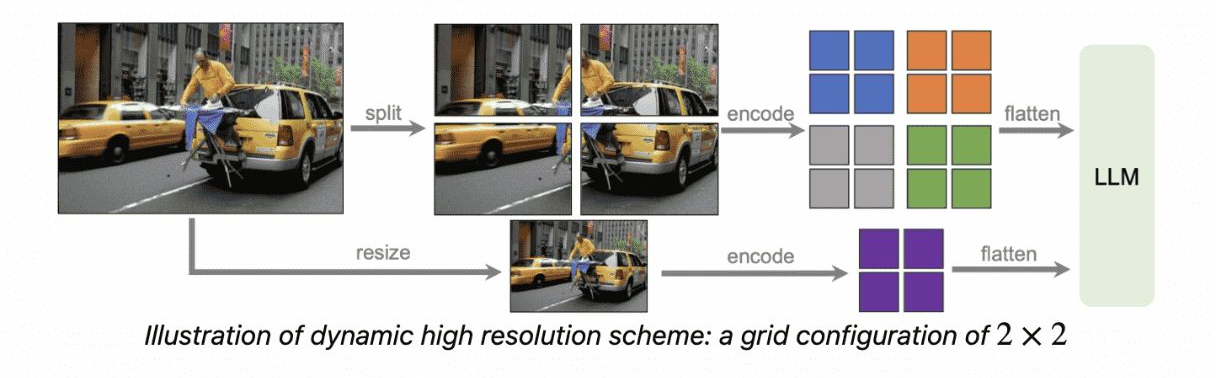
\includegraphics[width=0.98\textwidth]{images/2024-LLaVA-NeXT/fig-01.png}\end{center}
% source-block: XPFQd9SskoKz4XxXgwUc53Q8nfg
\par\vspace{0.95em}\noindent{\zihao{3}\bfseries 1.2 Data Mixture}\par\vspace{0.28em}
% source-block: TcXJdHByho15nPxFnBbcsia0nBh
\begin{itemize}
\item \textbf{High-quality User Instruct Data}：多样性，高质量回复
% source-block: IwbCd4JUMordrjxrpyPcJF5sn5B
\item \textbf{Multimodal Document/Chart Data}：模仿\href{https://huggingface.co/Qwen/Qwen-VL}{Qwen-VL-7B-Chat}增加了ChartQA
\end{itemize}
% source-block: BFutdXQvEoxeBAxMhFxcjqXqnQd
\par\vspace{0.95em}\noindent{\zihao{3}\bfseries 1.3 Scaling LLM backbone}\par\vspace{0.28em}
% source-block: XyVsdCpoqosKtGxwoaRcqylpnhb
In addition to Vicuna-1.5 (\href{https://huggingface.co/lmsys/vicuna-7b-v1.5}{7B} and \href{https://huggingface.co/lmsys/vicuna-13b-v1.5}{13B}), we consider more LLMs, including \href{https://mistral.ai/news/announcing-mistral-7b/}{Mistral-7B} and \href{https://huggingface.co/NousResearch/Nous-Hermes-2-Yi-34B}{Nous-Hermes-2-Yi-34B}.\par
% source-block: UnCAdUBOPor7UHxYTgecvEZGnNe
\clearpage
\par\vspace{1.15em}\noindent{\zihao{-2}\bfseries 2. Model Card}\par\vspace{0.28em}
% source-block: QoG7dvmyWozswix5ORoch4OjnDg
\begin{center}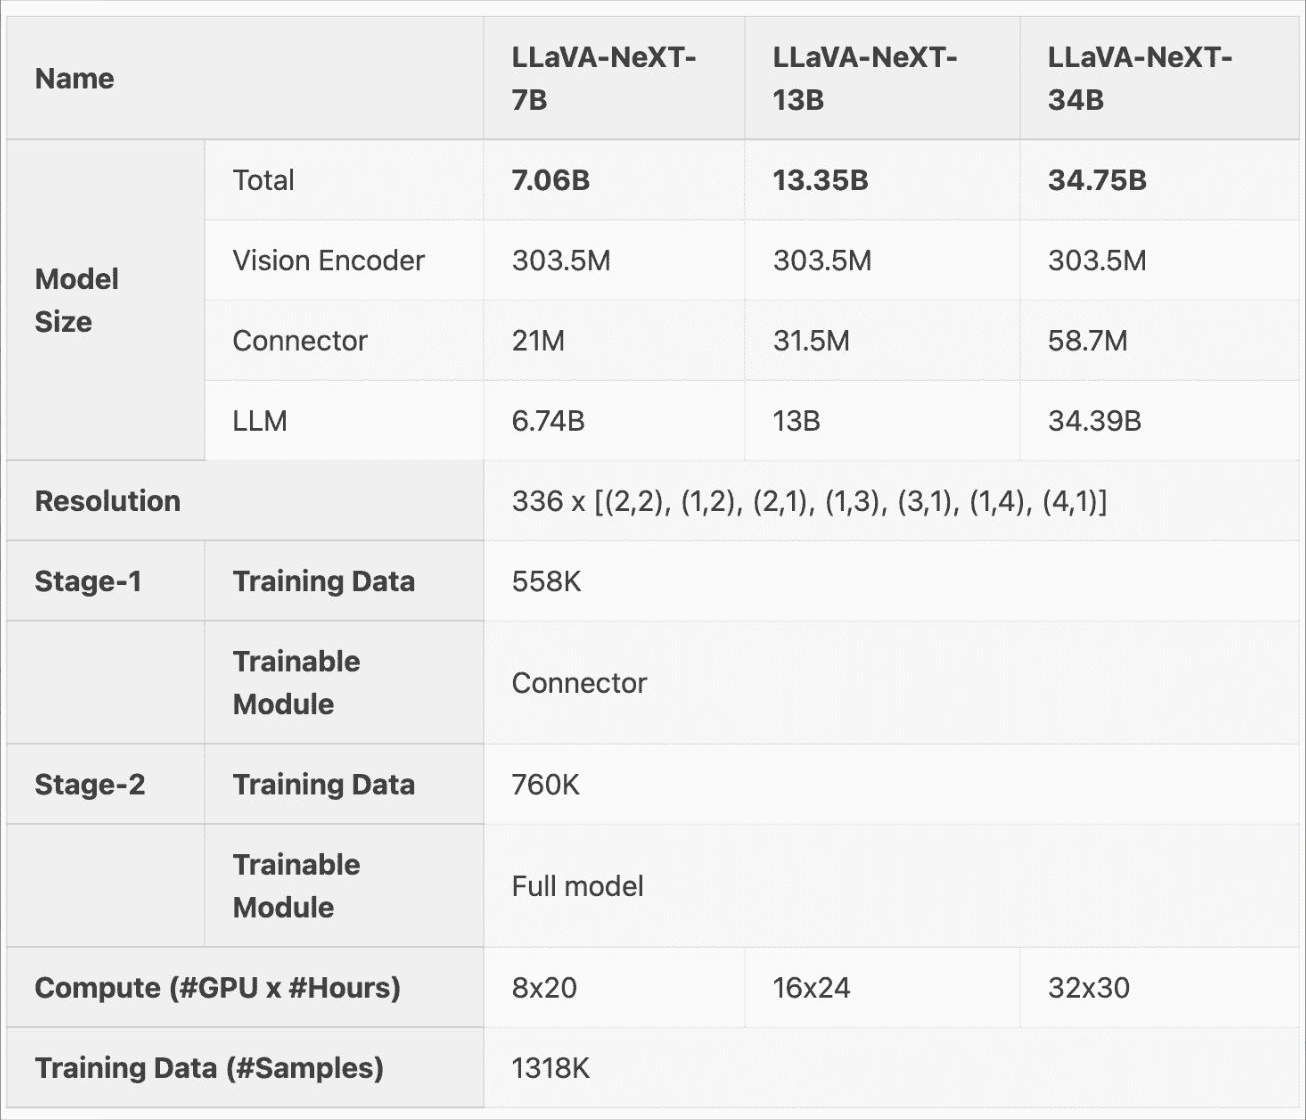
\includegraphics[width=0.98\textwidth]{images/2024-LLaVA-NeXT/fig-02.png}\end{center}
% source-block: Qg0RdSxmio3DTZxCgoFcO2iFnic
\begin{feishubox}{callSun}{🌟}
从LLaVA -{}-{}> LLaVA-1.5 -{}-{}> LLaVA-NeXT，\textbf{输入分辨率依次增大，视觉编码器能力、连接器能力、LLM基座能力更强，指令微调数据集包含更丰富、质量更高的数据集}\par
\end{feishubox}
% source-block: TISHd3PiboZoWvxSTPMc0K7Nn8c
\par\vspace{1.15em}\noindent{\zihao{-2}\bfseries Reference}\par\vspace{0.28em}
% source-block: R4Owd6qEeoZckRxCYfecRH2mnjf
[\textbf{1}]    LLaVA-NeXT: Improved reasoning, OCR, and world knowledge. \href{https://llava-vl.github.io/blog/2024-01-30-llava-next/}{https://llava-vl.github.io/blog/2024-01-30-llava-next/}\par
\end{document}
